\chapter{Figuras de mérito y evaluación}\label{cap.evaluacion}

Para evaluar de modo fiable la calidad de las redes neuronales profundas como predictores visuales se ha desarrollado una herramiento \textit{software} que obtienen unas figuras de mérito objetivas. El proceso de evaluación aplica las redes sobre los conjuntos de datos de test supervisados que se han descrito en el Capítulo~\ref{cap.generacion}, computa las figuras de mérito elegidas y las representa gráficamente para un mejor análisis. La comparación de estas gráficas de las distintas redes estudiadas es lo que permitirá extraer conclusiones sobre distintos parámetros.\\

En este capítulo se explican dichas figuras de mérito y se realiza un análisis en profundidad del código Python desarrollado para la evaluación, realizando también  una interpretación sobre los gráficos y resultados que arroja dicho código al terminar la ejecución.

\section{Figuras de mérito}

A continuación se describen las figuras de mérito que se han utilizado para evaluar las prestaciones de las redes, que se aplican tanto a imágenes modeladas como crudas. Para obtener conclusiones sobre la capacidad predictiva de las redes estudiadas se realiza una comparación entre dichas medidas. Estas comparaciones permiten obtener conclusiones sobre parámetros como el número de muestras utilizadas para entrenar, la complejidad de la dinámica o el horizonte temporal de predicción. Dichas conclusiones serán las que ayuden a tomar decisiones en la mejora del entrenamiento y la estructura de las redes para obtener la mejor red posible para la predicción.

\begin{description}
\item[Distancia entre píxeles] \hfill 
\vspace{10pt}
\\
La medida que se utiliza para cuantificar el error cometido en cada una de las predicciones es la distancia Euclídea\footnote{\url{https://en.wikipedia.org/wiki/Euclidean_distance}}  entre el píxel predicho~(\textit{p}) y el real~(\textit{q}). En dos dimensiones, su expresión viene dada por:  
$$d_E(p,q) = \sqrt{(p_1 - q_2)^2 + (p_1 - q_2)^2}$$

Además, para un  análisis más profundo, esta distancia se desglosa en cada una de las dimensiones de la imagen, \textit{x} e \textit{y}, simplemente calculando la diferencia en términos absolutos del valor en dichas coordenadas:
$$d_{E,dim}(p_{dim}, q_{dim}) = |p_{dim} - q_{dim}|$$

Las distancias anteriores cuantifican el error absoluto cometido en el plano de la imagen  y sus dimensiones \textit{x} e \textit{y}. Para analizar de una forma más completa la bondad de la red, se considera también el error relativo a la a la máxima distancia entre dos píxeles de la imagen, así como distintos estadísticos sobre las medidas de distancia.

\vspace{10pt}

\item[Distancia relativa] \hfill 
\vspace{10pt}
\\
La distancia absoluta puede dar una visión incompleta sobre el fallo que se ha cometido. Puesto que no es lo mismo desviarse una distancia de 5 píxeles en una imagen de 5x5 que en una de 1920x1080, se hace uso del error relativo\footnote{\url{https://en.wikipedia.org/wiki/Approximation_error}}. La medida relativa~($\eta$) normaliza la distancia absoluta~($\epsilon$) respecto a la máxima distancia en la imagen~($\upsilon$), haciendo uso de la siguiente fórmula:
$$\eta = \frac{\epsilon}{\upsilon}$$
En el caso de las imágenes, el máximo error a cometer es la mayor distancia entre dos píxeles de la imagen. Para una imagen de altura \textit{h} y anchura \textit{w}, la máxima distancia se corresponde con su diagonal, cuyo valor se obtiene de la siguiente manera:
$$\upsilon = \sqrt{h^2 + w^2}$$

La distancia relativa se suele indicar de forma porcentual, por lo que el valor calculado se multiplica por 100 para su expresión como porcentaje:
$$\delta = \eta * 100\%$$

La distancia relativa consigue normalizar la medida para una comparación más justa entre imágenes de distinto tamaño, permitiendo tener una idea más realista del fallo que se está cometiendo. 

\vspace{10pt}

\item[Estadísticos] \hfill 
\vspace{10pt}
\\
Para que la medición de la calidad de las predicciones sea fiable típicamente se aplica la red neuronal sobre un conjunto de secuencias, no sobre una única, es decir sobre varias secuencias supervisadas de fotogramas, que incluyen el fotograma verdadero en el tiempo de predicción. A partir de las medidas anteriores en dicho conjunto se obtienen una serie de estadísticos que permiten comparar las prestaciones de distintas redes y extraer conclusiones. A continuación se describen los estadísticos considerados.

\begin{itemize}
    \item \textbf{Máximo:} Se trata del error máximo cometido sobre todas las secuencias analizadas. Este valor identifica la imagen para la que más distancia existe entre la posición real y la predicha, que será uno de los elementos a tener en cuenta para examinar la bondad de la red. 
    \item \textbf{Media:} Se trata de la media de los vectores de error resultantes, absoluto y relativo, para obtener un único valor que permita hacer comparaciones rápidas.
\end{itemize}

\item[Formas de representación] \hfill 
\vspace{10pt}
\\
Para un mejor análisis de las figuras de mérito y los estadísticos presentados, se crean una serie de representaciones gráficas que contienen la información relevante para la comparación. Estas representaciones tienen su base en dos tipos:

\begin{itemize}
    \item \textbf{Histograma}\footnote{\url{https://en.wikipedia.org/wiki/Histogram}}: Se trata de un gráfico de barras que enfrenta la frecuencia con la que se comete un error con el valor del mismo, agrupado en intervalos para una representación más compacta.
    \item \textbf{\textit{Boxplot}}\footnote{\url{https://matplotlib.org/3.3.1/api/_as_gen/matplotlib.pyplot.boxplot.html}}: Se trata de un diagrama de caja y bigotes en el que la caja representa los cuartiles y las líneas que se extienden desde ella indican variabilidad fuera de los cuartiles superior e inferior. Por otro lado, los valores atípicos u \textit{outliers} se representan como puntos individuales dispersos por el eje vertical de la caja.
\end{itemize}

Todas las representaciones se combinan en una única figura, similar a la representada en la Figura~\ref{fig.test_example}, que se divide en cuatro regiones: una para el histograma del error absoluto, otra para el del relativo, una tercera para el \textit{boxplot} y la última con información de la media y el máximo. 

\begin{figure}[H]
		\begin{center}
			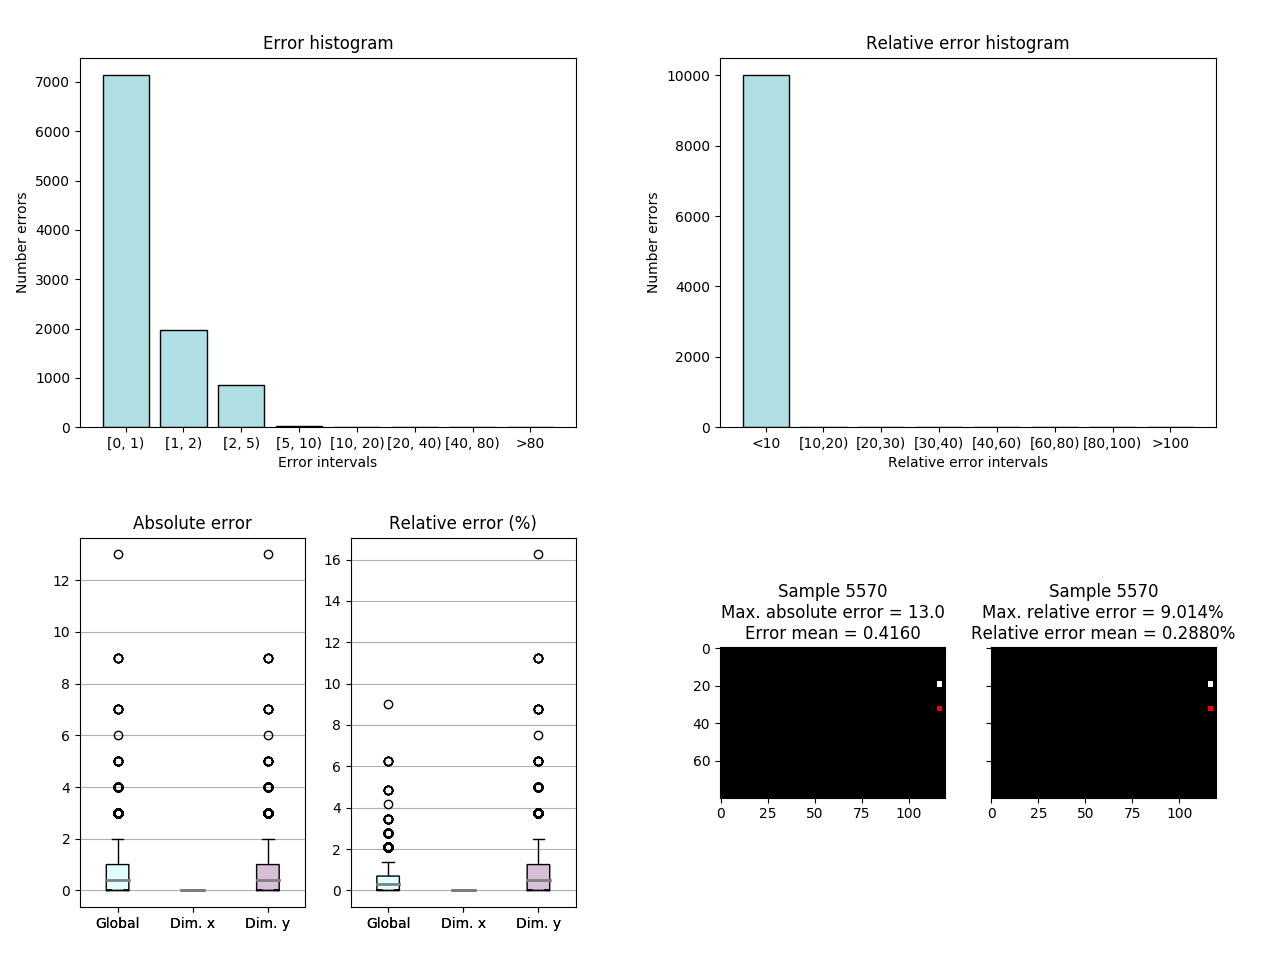
\includegraphics[width=0.9\textwidth]{ figures/error_stats_example.png}
			\caption{Ejemplo de gráfica con la distribución de distintas figuras de mérito y estadísticos asociados.}
			\label{fig.test_example}
		\end{center}
\end{figure}
\vspace{-10pt}

Con esta figura se representa de una forma resumida y clara toda la información referente las prestaciones de la red, a su calidad como predictor visual, facilitando la posterior tarea de análisis.
\vspace{10pt}
\end{description}

\section{Metodología de evaluación} \label{sec.eval}

Para el cálculo de las medidas  y la obtención de la Figura~\ref{fig.test_example} se ha desarrollado un código en Python sobre el que se profundiza en la siguiente sección.\\

En la Figura~\ref{fig.flujo_test} se muestra el flujo que sigue el código para evaluar una red concreta con un conjunto de \textit{test} determinado. El programa sigue un flujo muy sencillo y lineal cuyo resultado son la Figura~\ref{fig.test_example} y los valores asociados a las figuras de mérito que permiten la comparación de las distintas redes. 

\begin{figure}[H]
    \begin{center}
        \begin{tikzpicture}[node distance=2cm]
            \node (ld) [treenodelong] {Lectura de datos};
            \node (net) [treenodelong, below of=ld] {Carga de la red};
            \node (pred) [treenodelong, below of=net] {Predicción};
            \node (trans) [treenodelong, below of=pred] {Transformación de posiciones};    
            \node (calc) [treenodelong, below of=trans] {Cálculo de figuras de mérito};
            \node (pres) [treenodelong, below of=calc] {Presentación de resultados};
            
            \draw [arrow] (ld) -- (net);
            \draw [arrow] (net) -- (pred);
            \draw [arrow] (pred) -- (trans);
            \draw [arrow] (trans) -- (calc);
            \draw [arrow] (calc) -- (pres);
        \end{tikzpicture}
        \caption{Diagrama de flujo del evaluador.}
	    \label{fig.flujo_test}
	\end{center}
\end{figure}



En primer lugar se realizan las operaciones de lectura del conjunto de \textit{test} y carga de la red en memoria, cuyas rutas se obtienen del fichero de configuración correspondiente, para posteriormente pasar por la red los datos y obtener sus predicciones.\\

Puesto que las posiciones que se obtienen a la salida de la red tienen un formato diferente al de las posiciones reales, para obtener las figuras de mérito  es necesario realizar una transformación previa. Esta transformación dependerá del tipo de datos, modelados o crudos, que se estén tratando, ya que el problema se afronta de manera distinta en función de ello.

Cuando se trata con imágenes modeladas, se realiza una tarea de regresión. Es por ello que la salida de la red es un par de valores que corresponden a las coordenadas de la posición estimada. En este caso, la única acción a realizar es el redondeo de la estimación, para obtener un número entero. El procesamiento en el código queda de la siguiente manera:
\vspace{10pt}
\begin{lstlisting}[frame=single]
  p = np.round(p).astype(np.float64)
  predict_pos.append(p)
\end{lstlisting}
En el caso de trabajar con imágenes en crudo, el problema de predicción se aborda como un problema de clasificación binaria~(``0'' ó ``1'') donde la salida es un vector de longitud $h \times w$, con la codificación de la clase en cada píxel. En este caso se redimensiona el vector de salida al del tamaño de la imagen, obteniendo la posición del píxel activo de la siguiente forma:
\vspace{10pt}
\begin{lstlisting}[frame=single]
  p = p.reshape(dim)
  predict_pos.append(np.unravel_index(p.argmax(), p.shape))
\end{lstlisting}

Una vez obtenidas las posiciones predichas y reales en el mismo formato, se obtienen las figuras de mérito mediante el siguiente proceso:

\begin{enumerate}
    \item Se calcula, para cada imagen a predecir, la distancia entre la posición real del píxel activo y la estimada, es decir, el error absoluto.
    \item Se calcula el error relativo cometido, sobre el plano de imagen y las dimensiones \textit{x} e \textit{y}, en cada una de las imágenes a predecir.
    \item Se calculan los estadísticos para cada uno de los tipos de error obtenidos.
    \item Se crean los histogramas asociados al error absoluto y relativo en el plano de imagen.
    \item Se obtiene la imagen de máximo error, tanto absoluto como relativo, en el plano de imagen. Tras su identificación, se utilizan distintos colores para representar ambas posiciones (predicha y real) en una única figura.
    \item Se crea el \textit{boxplot} para los errores sobre el plano de la imagen, la dimensión \textit{x} y la dimensión \textit{y}. 
\end{enumerate}

Finalmente, tras el cálculo de las figuras de mérito y la creación de los gráficos que facilitarán la tarea de análisis, se almacenan los resultados en dos formatos distintos:
\begin{itemize}
    \item El fichero \textit{error}\_\textit{result.txt} almacena, para cada una de las imágenes predichas, el número que la identifica, la posición real, la posición predicha y los errores absoluto y relativo.
    \item Una figura que aúna cuatro gráficos representativos: los histogramas de los errores absolutos y relativos de cada imagen a predecir, el \textit{boxplot} de ambos tipos de error y la representación de la imagen de máximo error.
    
\end{itemize}

Con esta metodología para evaluar las prestaciones de una red se dispone de una forma objetiva de comparación entre redes, permitiendo  extraer conclusiones sobre distintos aspectos de las mismas.